%! TEX root = **/010-main.tex
% vim: spell spelllang=en:

\section{Feature score table}%
\label{sub:full-table-feature}

\begin{table}[H]
    \centering
    \caption{Score of all features}%
    \label{tab:features-all}
    \begin{tabular}{lr}
\toprule
                     Variable &     Score \\
\midrule
    \texttt{koi\_steff\_err1} &  0.189663 \\
           \texttt{koi\_prad} &  0.183599 \\
    \texttt{koi\_steff\_err2} &  0.179589 \\
 \texttt{koi\_duration\_err1} &  0.162258 \\
     \texttt{koi\_prad\_err2} &  0.156657 \\
     \texttt{koi\_prad\_err1} &  0.156133 \\
 \texttt{koi\_duration\_err2} &  0.152635 \\
     \texttt{koi\_model\_snr} &  0.140218 \\
     \texttt{koi\_srad\_err1} &  0.134092 \\
  \texttt{koi\_time0bk\_err1} &  0.129411 \\
         \texttt{koi\_period} &  0.128600 \\
  \texttt{koi\_time0bk\_err2} &  0.127128 \\
    \texttt{koi\_slogg\_err2} &  0.122820 \\
    \texttt{koi\_slogg\_err1} &  0.118122 \\
          \texttt{koi\_steff} &  0.115930 \\
   \texttt{koi\_period\_err2} &  0.110205 \\
    \texttt{koi\_insol\_err2} &  0.109296 \\
   \texttt{koi\_period\_err1} &  0.108270 \\
    \texttt{koi\_insol\_err1} &  0.105659 \\
          \texttt{koi\_depth} &  0.105383 \\
            \texttt{koi\_teq} &  0.102954 \\
         \texttt{koi\_impact} &  0.102895 \\
          \texttt{koi\_insol} &  0.102550 \\
           \texttt{koi\_srad} &  0.101156 \\
                 \texttt{dec} &  0.099278 \\
                  \texttt{ra} &  0.096536 \\
     \texttt{koi\_srad\_err2} &  0.094179 \\
          \texttt{koi\_slogg} &  0.092659 \\
    \texttt{koi\_depth\_err1} &  0.090870 \\
    \texttt{koi\_depth\_err2} &  0.090322 \\
         \texttt{koi\_kepmag} &  0.076024 \\
        \texttt{koi\_time0bk} &  0.072244 \\
   \texttt{koi\_impact\_err1} &  0.062623 \\
   \texttt{koi\_impact\_err2} &  0.055955 \\
 \texttt{koi\_tce\_plnt\_num} &  0.043661 \\
       \texttt{koi\_duration} &  0.022110 \\
\bottomrule
\end{tabular}

\end{table}

%\inputminted{cpp}{code.cpp}

%\subsection{Correlation Matrix}%


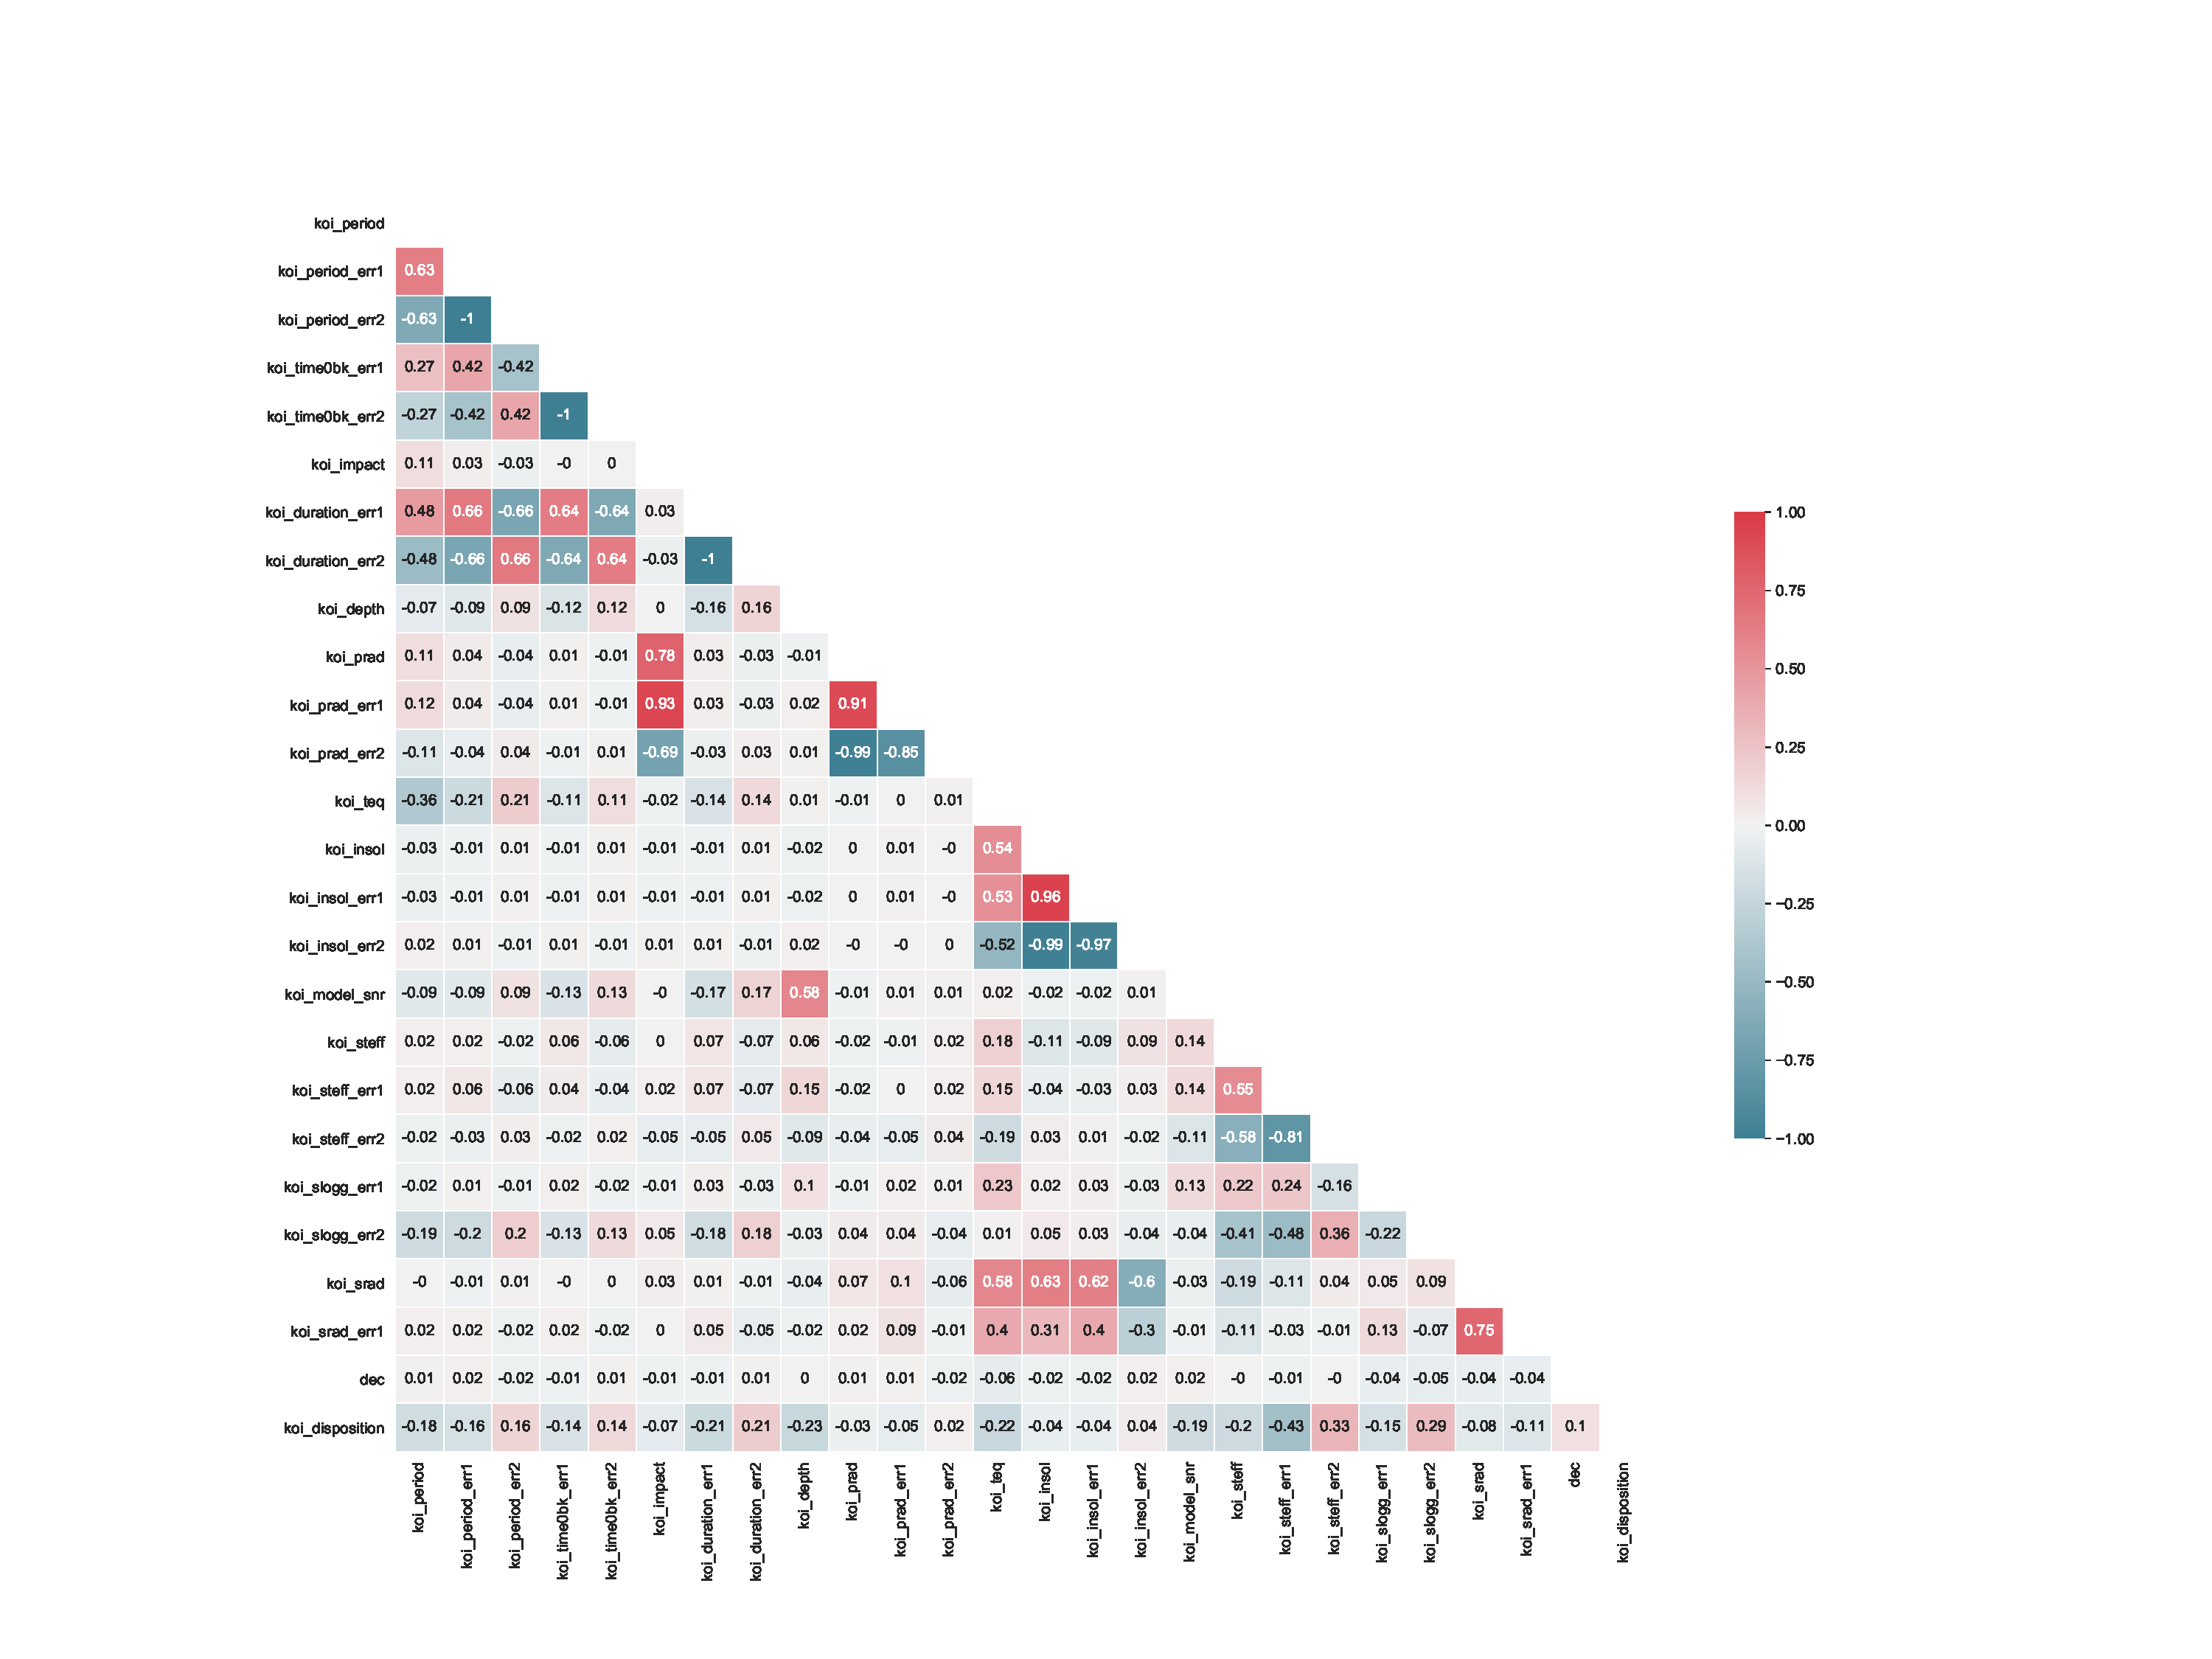
\includepdf[addtotoc={1,section,1,Correlation matrix,corr_mat}] {../figures/naive_bayes_correlation.pdf}
